%!TeX program = xelatex
\documentclass[12pt,hyperref,a4paper,UTF8]{ctexart}
\usepackage{NUDTReport}

%%-------------------------------正文开始---------------------------%%
\begin{document}

%%-----------------------封面--------------------%%
\cover
\thispagestyle{empty}
%%------------------摘要-------------%%
\newpage

\begin{center} 
  \fontsize{18pt}{16pt}
  \textbf{\selectfont 论文题目******}
\end{center}

\begin{center} 
  \textit{XXX}\textsuperscript{1}

  (1. \textit{国防科技大学 XXXX学院, 湖南 长沙}410073)
\end{center}

\begin{cnabstract}
%
  学术诚信即在逆境中坚守诚实、信任、公正、尊重和责任的价值观。尊重,学者间应相互尊重,尊重自我,诚实面对挑战尊重他人,重视观点的多样性欣赏挑战、检验和完善已有观点的必要性。信任,使学者能合作、共享信息,能自由地传播新思想,能使学术界之外的人相信学术研究、教学和学位(学历)授予的价值和意义。责任,学者个人和学术团体以身作则坚持共同认可的标准并在遇到错误时采取行动维护学术、教学和研究的诚信。公正,建立明确、公开的期望目标、评价标准和实践要求,以支持研究者和管理人员之间进行公正的交流。诚实,对待自己和他人对待数据和事实,对待已知和未知等学术研究的所有方面都应秉承坦诚的态度。

  \par\textbf{关键字: } 学术诚信;剽窃;引文
%
\end{cnabstract}

\begin{enabstract}
  Academic integrity means upholding the values of honesty, trust, justice, respect and responsibility in the face of adversity. Respect: Scholars should respect each other, respect themselves, face challenges honestly, respect others, value the diversity of viewpoints and appreciate the need to challenge, test and improve existing viewpoints. Trust enables scholars to collaborate, share information, disseminate new ideas freely, and convince those outside academia of the value and significance of academic research, teaching, and the awarding of degrees. Individual academics and academic communities lead by example to uphold commonly agreed standards and take action when errors are encountered to uphold the integrity of scholarship, teaching and research. Establish clear and public expectations, evaluation criteria, and practice requirements to support impartial communication between researchers and administrators. Be honest, be honest with yourself and others about data and facts, about the known and the unknown, about all aspects of academic research.
  \par\textbf{Keywords:} Academic integrity; Plagiarism; quotation
  %“\par在段首,表示另起一行,“\textbf{}”,花括号内的内容加粗显示
\end{enabstract}

\thispagestyle{empty} % 首页不显示页码

%%--------------------------目录页------------------------%%
\newpage
\tableofcontents
\thispagestyle{empty}

%%------------------------正文页从这里开始-------------------%

\newpage
\setcounter{page}{1}
%%可选择这里也放一个标题
%\begin{center}
%    \title{ \Huge \textbf{{标题}}}
%\end{center}

\section{引言}
学术活动中诚实守信,即实事求是、不欺骗、不弄虚作假,恪守科学精神、学术规范。科学精神(学术精神):学术研究主体所恪守的学术信念与操守。现代学术精神的要素:独立精神、自由精神、怀疑精神、反思精神、规范观念、批判态度等。

学术诚信即在逆境中坚守诚实、信任、公正、尊重和责任的价值观。尊重,学者间应相互尊重,尊重自我,诚实面对挑战尊重他人,重视观点的多样性欣赏挑战、检验和完善已有观点的必要性。信任,使学者能合作、共享信息,能自由地传播新思想,能使学术界之外的人相信学术研究、教学和学位(学历)授予的价值和意义。责任,学者个人和学术团体以身作则坚持共同认可的标准并在遇到错误时采取行动 维护学术、教学和研究的诚信。公正,建立明确、公开的期望目标、评价标准和实践要求,以支持研究者和管理人员之间进行公正的交流。诚实,对待自己和他人对待数据和事实,对待已知和未知等学术研究的所有方面都应秉承坦诚的态度。

\begin{figure}[!htbp]
  \centering
  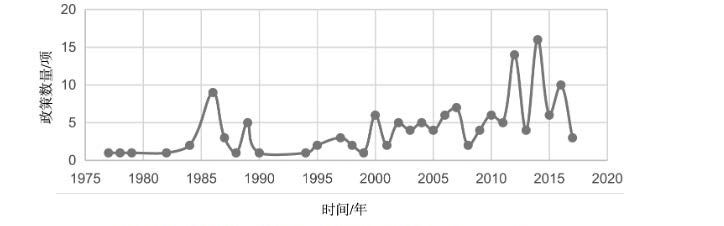
\includegraphics[width = 14cm]{figures/fig1.jpg}
    \caption{我国国家层面科研诚信政策的年度数量分布(1949-2017)\textsuperscript{\cite{GongHaoJiYuWenBenWaJueDeWoGuo20022021NianKeYanChengXinZhengCeBianQianTeZhengFenXi2022}}}
    \label{数量分布}
\end{figure}

由图1可知,我国国家层面科研诚信政策的年度数量分布主要呈现出三个阶段\textsuperscript{\cite{GongHaoJiYuWenBenWaJueDeWoGuo20022021NianKeYanChengXinZhengCeBianQianTeZhengFenXi2022}},由以下组成:
\begin{itemize}
    \item \texttt{未显期(
    1949-1986)} 
    
    特征:科研诚信问题不明显,鲜有发生,个别诚信事件及时处理。政策:以建设性规则为主从正面完善科研活动的社会环境。 政策中出现了科研诚信要素。问题:学术不端主要通过举报、投诉。

    \item \texttt{渐显期(
    1987-2011)} 
    
    特征:问题逐步显现,引起科研界重视,部
    分事件引发社会公众关注。政策:首次出现针对科研诚信的专项政策,新制度新方法从正反面遏制负面问题。问题:学术不端主要表现为造假、抄袭、一稿多投多发等。媒体关注引发负面舆情。

    \item \texttt{凸显期(
    2012-至今)} 
    
    特征:问题尖锐,群体性撤稿等事件频发,引发广泛关注,对科研环境产生负面影响,治理力度大为提升。政策:相关政策数量显著提升、政策所涉对象显著深化、联手政策部门显著增多、对负面行为的惩戒细化并强调可操作性。问题:信息技术的应用提升抄袭问题发现,突出表现为评议操纵、数据 图像造假、不可复现,以及科学伦理问题等。
 
\end{itemize}

面对科研诚信问题,2018年,中共中央办公厅、国务院办公厅出台了《关于进一步加强科研诚信建设的若干意见》\textsuperscript{\cite{ShiLuYanZhongGongZhongYangBanGongTingGuoWuYuanBanGongTingYinFaGuanYuJinYiBuJiaQiangKeYanChengXinJianSheDeRuoGanYiJian}}这一指导性文件,对科研诚信问题提出了“全覆盖、无禁区、零容忍”的治理原则,确立了自上而下、覆盖全面的科研诚信建设的责任体系。在2021 年 5 月 28 日,习近平主席在中国科学院第二十次院士大会、中国工程院第十五次院士大会、中国科协第十次全国代表大会上的讲话“诚信是科学精神的必然要求”。作为国家战略科技力量主力军,国防科技大学始终将科研诚信建设当作一项长期任务,用持之以恒的决心、行之以稳的坚持,营造诚信文化,建设优良学风。五年来,陆续发布科研诚信提醒的方式,突出重点、层层深入地不断筑牢科研诚信的基石,营造风清气正的学术氛围。如今,全院上下已经形成了思想高度重视、体系相对完善、工作各负其责、案件查办“零容忍”的良好局面。

科技自立自强是国家强盛之基、安全之要,而要实现高水平科技自立自强必须筑牢科研诚信的基石。学校学院持续关注科研诚信、学风建设话题。本文对科研诚信话题进行延展报道,对可能出现的科研诚信提醒进行梳理,多方位展示学院领到专家对科研诚信、学风建设的真知灼见,为坚守科研诚信底线、营造优良学风提供多维度建议。

\section{常见科研失信行为与案例研究}
\subsection{剽窃行为及案例研究}
\subsubsection{剽窃行为定义与表现}
剽窃,即采用不当手段,窃取他人的观点、数据、图像、研究方法、文字表述等并以自己名义发表的行为\textsuperscript{\cite{学术出版规范——期刊学术不端行为界定(CY/T1742019)}}。主要的表现形式有以下几种:

1.观点剽窃: 不加引注或说明 地使用他人的 观点 ,并以自己的名义发表。

2.数据剽窃: 不加引注或说明 地使用他人已发表文献中的 数据 ,并以自己的名义发表。

3.图片和音视频剽窃 不加引注或说明 地使用他人已发表文献中的 图片和音视频 ,并以自己的名义发表。

4.研究 (实验) 方法剽窃

5.文字表述剽窃

6.整体剽窃:论文的主体或论文某一部分的主体过度引用或大量引用他人已发表文献的内容,应界定为整体剽窃。

7.他人未发表成果剽窃

8.自我剽窃:重新使用自己以前已经公开发表的研究成果而未在参考文献中明确引用。

\subsubsection{剽窃行为案例研究}

几乎一字不差的硕士学位论文抄袭事件:2016
年 1 月底,上海媒体“澎湃新闻”( www thepaper.cn )和四川的 《 华西都市报 》 先后刊发报道,揭
露两篇金融学专业的硕士学位论文高度相似雷同,存在学术造假嫌疑。其中,一篇论文的作者是东北师范大学金融学专业硕士毕业生张强,其论文题目是“我国货币政策对股票市场的效应研究”,另一篇的作者是西南财经大学金融学专业硕士毕业生杨某,其论文题目为“我国货币政策对股票市场的效应研究”。

张强的学位论文完成于2009 年 5 月 1 日,而杨某的学位论文则完成于 2009 年 12 月 1 日。就完成时间来看,张强的论文在前,杨某的论文在后,两篇论文的完成时间前后相差大约半年。

这两篇论文不仅在结构、目录上完全一样,在主体的正文部分,从各章节的大小标题到具体内容的文字叙述,基本都完全一致。正如报道所说,对比两篇论文,“要找出不一样的地方,才是真正的困难之处”。很明显,两篇论文中必有一篇抄袭了另一篇,属于 严重的学术不端为。西南财经大学在 2014 年 取消了杨某的硕士学位。

由此可见,论文剽窃的后果很严重。对于学生,剽窃行为可能会导致课程不及格甚至撤销学位;
对于研究学者则会危及职业和声誉,为侵犯版权承担法律责任和行政责任。

\subsection{伪造行为及案例研究}
\subsubsection{伪造行为定义与表现}
在科学研究活动中,记录或报告无中生有的数据或实验结果的一种结果\textsuperscript{\cite{学术出版规范——期刊学术不端行为界定(CY/T1742019)}}。表现形式:

1.
编造 不以实际调查或实验取得的数据、图片等。

2.
伪造无法通过重复实验而再次取得的样品等。

3.
编造 不符合实际或无法重复验证的研究方法、结论等。

4.
编造 能为论文提供支撑的资料、注释、参考文献。

5.
编造 论文中相关研究的资助来源。

6.
编造 审稿人信息、审稿意见。

\subsubsection{伪造行为案例研究}

2014年8月,日本理化学研究所(Riken)的发育生物学中心(CDB)副主任笹井芳(Yoshiki Sasai)在位于神户市的该中心内自杀身亡,他被誉为日本离诺贝尔奖最近的科学家。2014年1月,他的学生小保方晴子在《自然》杂志发表了两篇关于多能干细胞的论文。两篇文章是关于“刺激触发的多能获得性”(STAP)技术的,在文章中,小保方晴子声称只需运用一种简单的方法,就能够让小鼠的体细胞变成干细胞。然而,文章发表数周后。美国科学家指出了其中的造假数据其他科学家也表示不能重复试验结果。研究所的一个委员会经过调查之后,在当年4月1日正式指控小保方晴子的不端行为,并提议撤销该论文2014年7月,两篇文章随即被撤销。8月,不堪多重压力的笹井芳树选择了自杀。12月19日,日本理化学研究所召开记者会,就STAP细胞制备论文造假事件的结果做出最后说明。会上公布了小保方晴子在全程监控的状态下重复自己先前实验的结果,数据显示原论文中“成功制备”的STAP嵌合体胚胎一个都没有制备出来。根据先前规定的期限,实验就此终止。小保方晴子本人没有出现在记者会上,但发布了公开信,并主动提出辞职。

\subsection{篡改行为及案例研究}
\subsubsection{篡改行为定义与表现}
在科学研究活动中,操纵 实验材料、设备或实验步骤, 更改或省略 数据或部分结果使得研究记录不能真实地反映实际情况的一种行为\textsuperscript{\cite{学术出版规范——期刊学术不端行为界定(CY/T1742019)}}。表现形式:

1.使用经过擅自修改、挑选、删减、增加的原始调查记录、实验数据等,使原始调查记录、实验数据等的本意发生改变。

2.拼接不同图片从而构造不真实的图片。

3.从图片整体中去除一部分或添加一些虚构的部分,使对图片的解释发生改变。

4.增强、模糊、移动图片的特定部分,使对图片的解释发生改变。

5.改变所引用文献的本意,使其对己有利。

\subsubsection{篡改行为案例研究}

国家自然科学基金委员会监督委员会对山东大学周某斌等发表的论文Fang Xue, Haibin Zhou* et al. MicroRNA 139 3p inhibits the growth and metastasis of ovarian cancer by inhibiting ELAVL1. OncoTargets and Therapy, 2019, 12: 8935-8945.(标注基金号30901987)涉嫌学术不端开展了调查。经查,涉事论文的实验部分由第一作者薛某委托第三方公司完成作者对实验数据的真实性疏于审核,造成伪造篡改实验数据的客观结果,薛某和通讯作者周某斌应对上述问题负责。此外周某斌将论文列入基金项目(申请号8217060643)申请书,还应对基金项目申请书中存在虚假信息的客观结果负责。经国家自然科学基金委员会监督委员会六届一次会议审议,国家自然科学基金委员会2023年第13次委务会议审定,决定依据《国家自然科学基金项目科研不端行为调查处理办法》第四十七条、第四十条,撤销周某斌国家自然科学基金项目Sirt1在白藜芦醇诱导成骨细胞分化中的作用机制研究(批准号30901987追回已拨资金取消周某斌国家自然科学基金项目申请和参与申请资格3年2023年8月21日至2026年8月20日),给予通报批评。

PubPeer建立于2012年,是一个鼓励科研人员匿名对已发表的论文进行评论的网站,目前评论存在学术造假嫌疑的论文已多达数十万篇,平均每年曝光1万余篇,中国、美国、日本、伊朗、印度是曝光数量最多的国家,其中绝大部分论文来自生命科学领域。PubPeer学术打假最开始的逻辑是查找图像相似度。图像的相似度较高的情况有图像的复制、颠倒、翻转、部分重叠等,这些情况通常是由于论文作者对图像进行人为操纵,一图多用导致的。2020年,Pubpeer上挂出2019年诺贝尔生理学或医学奖得主格雷格·塞门扎(Gregg L. Semenza)的争议论文达40篇,时间跨度长达18年。这些论文被质疑一图多用或图片PS,少数文章还被质疑存在伦理问题。Gregg L. Semenza教授主要从事低氧诱导因子(HIF)相关领域研究,被曝有问题的论文不在其中已发表论文600余篇,被引用超过16万次。诺贝尔奖官方网站上公示的两篇“关键著作”没有被打假。

\subsection{不当署名行为及案例研究}
\subsubsection{不当署名行为定义与表现}
指署名与对论文的实际贡献不符\textsuperscript{\cite{学术出版规范——期刊学术不端行为界定(CY/T1742019)}}。表现形式:

1.
将对论文研究内容有实质性贡献的人排除在作者名单外。

2.
未对论文所涉及的研究有实质性贡献的人在论文中署名。

3.
擅自在自己的论文中加署他人的姓名。

4.
虚假标注作者信息,如提供虚假的作者职称、单位、学历、研究经历等信息。

5.
作者排名不能正确反映实际贡献。

\begin{figure}[!htbp]
    \centering
    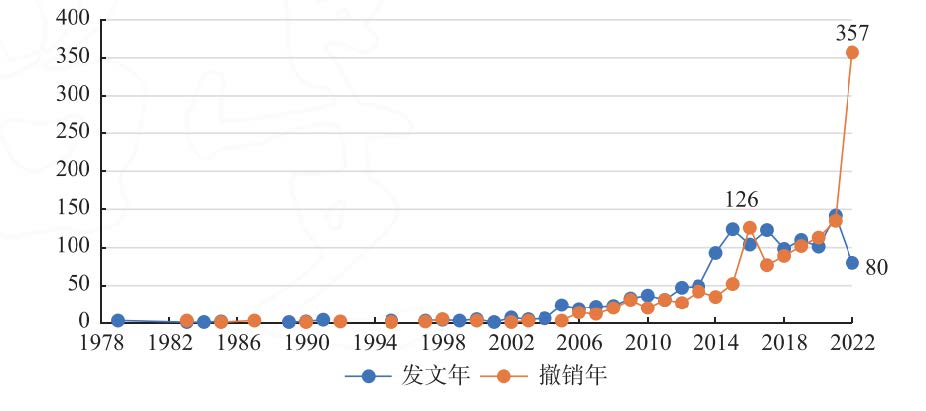
\includegraphics[width =14cm]{figures/fig2.jpg}
    \caption{因署名问题撤销论文的时间分布\textsuperscript{\cite{FengLingZiShuMingWenTiZhongHuiSeDiDaiKeYanBuDuanXingWeiDeFangFanYuZhiLiJiYuCheXiaoLunWenDeFenXi2023}}}
    \label{署名问题}
\end{figure}

\subsubsection{不当署名行为案例研究}

2022年,北大一研究生偷取了同门师妹的论文发表,作者栏却写的是武大3名研究生的名。其目的是为了毁掉同门师妹的这篇论文。2个月后,这篇严重涉嫌学术不端的论文被杂志出版商以使用了虚假的作者详细信息为由撤回了。不过被挂名的3位武大研究生,也是接受了一段时间的调查。

2023年原首都医科大学附属北京同仁医院(简称北京同仁医院)内分泌科主任杨某奎向澎湃科技表示,在他向相关学术期刊持续申诉近半年后,他“被署名”的5篇论文目前已撤回3篇。起因是他发现自己明明没有参与上述论文的研究,但名字出现在涉事论文的作者一栏中,并被列为通讯作者之一。

\subsection{一稿多投行为及案例研究}
\subsubsection{一稿多投行为定义与表现}
指将同一篇论文或只有微小差别的多篇论文,投给多个期刊,或在约定或法定期限内再转投其他期刊\textsuperscript{\cite{学术出版规范——期刊学术不端行为界定(CY/T1742019)}}。表现形式:

1.将同一篇论文同时投给多个期刊。

2.在首次投稿的约定回复期内,将论文再次投给其他期刊。

3.在未接到期刊确认撤稿的正式通知前,将稿件投给其他期刊。

4.将只有微小差别的多篇论文,同时投给多个期刊。

5.在收到首次投稿期刊回复之前或在约定期内,对论文进行稍微修改后,投给其他期刊。

6.在不做任何说明的情况下,将自己(或自己作为作者之一)已经发表论文,原封不动或做些微修改后再次投稿。指将同一篇论文或只有微小差别的多篇论文,投给多个期刊,或在约定或法定期限内再转投其他期刊。

\subsubsection{一稿多投行为案例研究}

2018年10月24日,《中国青年报》刊出一篇题为《青年长江学者与她“404”的论文》,在学术界和舆论场上掀起了一场风暴。文章揭露:在过去几年里南京大学教授梁某,主动将她的这些中文论文从中国知网、万方、维普等主要学术期刊数据库删除。经调查,梁某的至少有15篇论文涉嫌抄袭、一稿多投等学术不端问题,并在教学工作中存在敷衍怠慢的问题。

2018年12月12日,南京大学给予梁某党内严重警告处分、行政记过处分,取消梁某研究生导师资格,将其调离教学科研岗位,终止“长江学者奖励计划”青年学者聘任合同;报请上级有关部门撤销其相关人才计划称号和教师资格。

2018年12月30日,从教育部获悉,教育部已按程序撤销梁某的“青年长江学者”称号。

%\section{定理环境}
%\begin{Theorem}
%\end{Theorem}
%
%\begin{Lemma}
%\end{Lemma}
%
%\begin{Corollary}
%\end{Corollary}
%
%\begin{Proposition}
%\end{Proposition}
%
%\begin{Definition}
%\end{Definition}
%
%\begin{Example}
%\end{Example}
%
%\begin{proof}
%\end{proof}

\subsection{重复发表行为及案例研究}
\subsubsection{重复发表行为定义与表现}
指作者向不同出版机构投稿时,其文稿内容与已发表论文内容雷同且缺乏充分的交叉引用的现象\textsuperscript{\cite{学术出版规范——期刊学术不端行为界定(CY/T1742019)}}。表现形式:

1.
不加引注或说明,在论文中使用自己(或自己作为作者之一)已发表文献中的内容。

2.
在不做任何说明的情况下,摘取多篇自己(或自己作为作者之一)已发表文献中的部分内容,拼接成一篇新论文后再次发表。

3.
被允许的二次发表不说明首次发表出处。

4.
不加引注或说明地在多篇论文中重复使用一次调查、一个实验的数据等。

5.
将实质上基于同一实验或研究的论文,每次补充少量数据或资料后,多次发表方法、结论等相似或雷同的论文。

6.
合作者就同一调查、实验、结果等,发表数据、方法、结论等明显相似或雷同的论文。

\subsubsection{重复发表行为案例研究}
2018年10月,媒体报道清华大学有11篇材料科学领域的论文,由于图片篡改、内容重复、虚假署名等学术不端行为而遭撤稿。这些论文的发表时间为2014年到2016年,通讯作者是清华大学深圳先进研究院能源与环境部常务副所长唐某翌教授,第一作者均为叶某鑫。叶某鑫是唐某翌指导的10级博士生,2015年7月毕业并获清华大学博士学位。在5年的读博期间,叶某鑫以一作发表论文16篇,曾获清华学术新秀提名,还担任几个知名SCI期刊编辑和审稿人。但据媒体报道,他高产的背后,竟是不断地重复使用自己的图片与数据。

2018年10月21日,清华大学深圳研究生院发布“关于对叶某鑫学术不端问题调查处理情况的说明”称“2017年4月,我院已会同学校有关部门,对叶某鑫涉及严重学术不端的问题进行了严肃处理,撤销其博士学位,同时对其导师追责问责。”清华大学深圳研究生院还表示2017年6月,停止唐某翌教授招收研究生资格,撤销其材料学科负责人和新材料研究所副所长职务。

\subsection{违背研究伦理行为及案例研究}
\subsubsection{违背研究伦理行为定义与表现}
论文涉及的研究未按规定获得伦理审批,或者超出伦理审批许可范围,或者违背研究伦理规范\textsuperscript{\cite{学术出版规范——期刊学术不端行为界定(CY/T1742019)}}。表现形式:

1.
论文所涉及的研究未按规定获得相应的伦理审批,或不能提供相应的审批证明。

2.
论文所涉及的研究超出伦理审批许可的范围。

3.
论文所涉及的研究中存在不当伤害研究参与者,虐待有生命的实验对象,违背知情同意原则等违背研究伦理的问题。

4.
论文泄露了被试者或被调查者的隐私。

5.
论文未按规定对所涉及研究中的利益冲突予以说明。

\subsubsection{违背研究伦理行为案例研究}

2016年6月开始,南方医科大学副教授贺建奎私自组织包括境外人员参加的项目团队,蓄意逃避监管,使用安全性、有效性不确切的技术,实施国家明令禁止的以生殖为目的的人类胚胎基因编辑活动。2017年3月至2018年11月,贺建奎通过他人伪造伦理审查书,招募8对夫妇志愿者艾滋病病毒抗体男方阳性、女方阴性参与实验。为规避艾滋病病毒携带者不得实施辅助生殖的相关规定,策划他人顶替志愿者验血,指使个别从业人员违规在人类胚胎上进行基因编辑并植入母体,最终有2名志愿者怀孕,其中1名已生下双胞胎女婴“露露”“娜娜”,另1名在怀孕中。其余6对志愿者有1对中途退出实验,另外5对均未受孕。该行为严重违背伦理道德和科研诚信,严重违反国家有关规定,在国内外造成恶劣影响。2019年,南方医科大学研究决定:解除与贺某奎的劳动合同关系,终止其在校内一切教学科研活动。在同年,此人也因非法实施人类胚胎基因的研究而被法院追究刑事责任,判处有期徒刑三年再加三百万罚款。

\subsection{其他的科研不端行为}
1.
将转引自其他文献的引文标注为直引,包括将引自译著的引文标注为引自原著。

2.
未以恰当的方式,对他人提供的研究经费、实验设备、材料、数据、思路、未公开的资料等,给予说明和承认(有特殊要求的除外)。

3.
不按约定向他人或社会泄露论文关键信息,侵犯投稿期刊的首发权。

4.
未经许可,使用需要获得许可的版权文献。

5.
使用多人共有版权文献时,未经所有版权者同意。

6.
经许可使用他人版权文献,却不加引注,或引用文献信息不完整。

7.
经许可使用他人版权文献,却超过了允许使用的范围或目的。

8.
在非匿名评审程序中干扰期刊编辑、审稿专家。

9.
向编辑推荐与自己有利益关系的审稿专家。

10.
委托第三方机构或者与论文内容无关的他人代写、代投、代修 。

11.
违反保密规定发表论文。


\section{学位论文和学术论文撰写规范}

学术规范,即学术共同体成员必须遵守的准则,是保证学术共同体科学、高效、公正运行的条件,它在学术活动中约定俗成地产生,并称为相对独立的规范系统。

根据中华人民共和国国家标准《科学技术报告、学位论文和学术论文的编写格式》《中华人民共和国保守国家秘密法》和《中国人民解放军保密条例》,以及国务院学位委员会和学校的有关要求,为进一步规范学位论文格式,提高学位论文的撰写质量,特制定本规定。

学术学位硕士论文应是一篇系统而完整的学术论文。学位论文的基本论点、结论和建议,应有一定的学术价值或对国民经济建设具有一定的理论和实践意义;论文内容应体现出作者具有坚实的基础理论和系统的专门知识;应反映出科学的研究方法和较熟练的技能;应具有新的见解并取得一定的科研或技术成果。

\subsection{学术论文致谢的要求}
位置:在正文后、参考文献前或论文首页的脚注。

\begin{itemize}
	\item 致谢对研究或论文提出过建议和帮助的个人和机构并指出被谢者的工作内容和贡献。
	\item 标明研究的基金来源,比如 Nature Science Foundation of China(NSFC,国家自然科学基金),并标注基金号码(Grant Number)。
\end{itemize}

\subsection{学术引文规范引}

引文(参考文献):为了撰写或编辑论著而引用或参考的有关文献资料,通常附在论文、图书或每章、节之后有时也以注释(附注或脚注)形式出现在正文中。
引文是学术论著的重要组成部分,它表明文献之间的继承和发展关系。

引用的原因:
\begin{itemize}
	\item 起源
	\item 提供证据和说明
	\item 提供背景阅读资料
	\item 评价或更正以前的观点
\end{itemize}

\subsubsection{引文使用的原则}
(1)不能引而不用,不选而引

伪引(伪注):并未引用别人的成果,但却将该成果列在注释或参考文献中。包括将转引标注为直引。

(2)不能用而不引 (漏引、直接引用、间接引用、转引、自引)

漏引:引用了别人的成果,但是未在参考文献注明,或虽然列出参考文献,但是行文中未明确注明哪些是别人或自己的。

直接引用:引用的部分一字不改地照录原话,引文前后加引号。

间接引用(暗引):吸收了别人的成果,但用自己的语句表述。多用于原文过长、常识性资料等。

转引:自己未阅读原始文献,只根据二手资料、译文或他人引用的资料加以引用。在引用文献中列出中介文献和原始文献、只列出中介文献、只列出出原始文献。

自引(自我引用):指著者引用自己已发表的著作或与他人合著的著作。引文以正式或审核过的文献为主;引用文献有多个版本时,应注意引用恰当的版本文献;忠实原著,不能断章取义;引自中译本,只标注中译本;间接引文也应列入参考文献中,并标明出处、页码;不能过度引用,抄袭。

过度引用:超过了适度引用范围,引用他人的作品构成了自己作品的主要部分或实质部分的引用行为。实质就是抄袭。

\subsubsection{学术论文写作引用图片原则}
\noindent1、\textbf{获得版权授权}
(引用自己发表的论文图片)

\noindent2、\textbf{标注来源和版权信息}

在图片下方注明图片来源、版权信息和引用日期等。

\noindent3、\textbf{保持图片质量}

\noindent4、\textbf{遵守引用规范}

\noindent5、\textbf{注意图片版面设计}

与论文的主题相关,图片的大小、分辨率和格式等符合期刊的要求。

\subsubsection{引文著录的要求}

\begin{itemize}
	\item 信息与文献参考文献著录规则 (GB/T 7714-2015)
	
	\begin{figure}[!htbp]
      \centering
      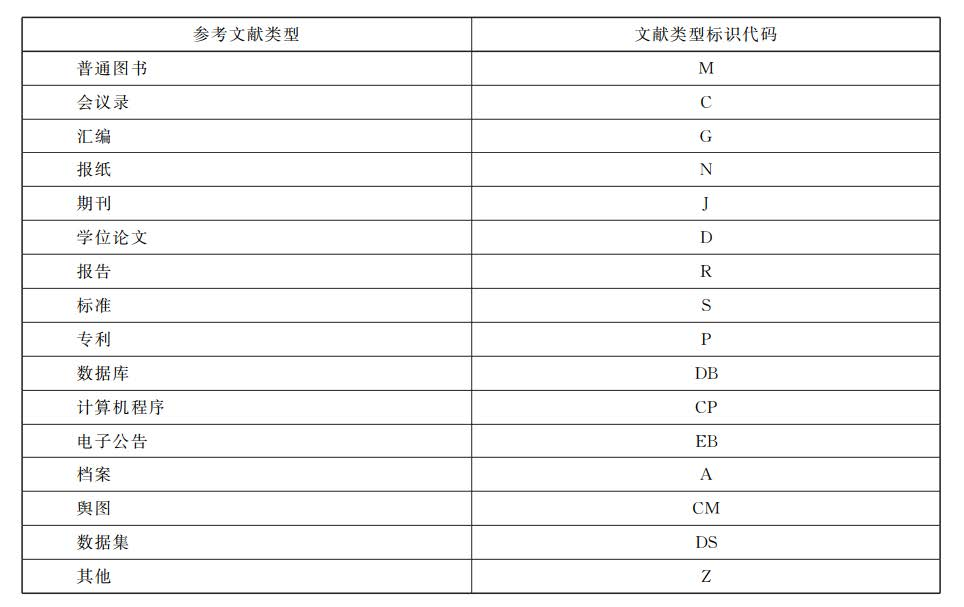
\includegraphics[width =14cm]{figures/fig3.jpg}
      \caption{参考文献著录规则 (GB/T 7714-2015)}
      \label{参考文献}
  \end{figure}

	\item 芝加哥(图拉宾式)
	\item 现代语言协会( MLA ):人文学科
	\item 美国心理学协会( APA ):社会科学、教育学、工程学和商学
	\item 自然学科自己独特的引注规则
\end{itemize}

例如:


   \textit{ 此处引用了文献\textsuperscript{\cite{学术出版规范——期刊学术不端行为界定(CY/T1742019)}}。此处引用了文献\textsuperscript{\cite{FengLingZiShuMingWenTiZhongHuiSeDiDaiKeYanBuDuanXingWeiDeFangFanYuZhiLiJiYuCheXiaoLunWenDeFenXi2023}}}

参考文献原则上要求用信息资源本身的语种著录。 必要时 , 可采用双语著录。 用双语著录参考文献时 , 首
先应用信息资源的原语种著录 , 然后用其他语种著录。

著录用符号为前置符,即根据其后面的内容确定使用什么符号。

著作方式相同的责任者不超过 3 个时 , 全部照录。 超过 3 个时 , 著录前 3 个责任者 , 其后加“ “, 等”

无责任者或者责任者情况不明的文献 , 主要责任者”项应注明“佚名”或与之相应的词。

标点使用英文格式。

\section{结论}

在学术规范的报告中,我们深入探讨了学术研究中的伦理要求、写作规范以及学术诚信等重要议题,对于我作为一名研究生而言,这是一次极具启发性的经历。

在研究过程中,我们必须始终遵循学术道德,诚信地开展研究工作。这意味着不仅要尊重他人的知识产权,还要保持数据的准确性和可信度,杜绝学术不端的行为。同时,对于已有文献的引用和使用,也要遵循严格的规范,确保学术成果的真实性和可追溯性。学术写作应该注重准确性和清晰度。在表达观点和研究成果时,要注意语言的精确性,避免模糊和含糊不清的表达。此外,对于文献的引用和参考,也需要遵循相应的引用规范,确保信息的完整性和可查性。学术规范的重要性不仅体现在研究过程中,也反映在学术成果的评价和认可上。只有遵循规范,才能够获得同行的认可和尊重,进而为自己的学术生涯奠定坚实的基础。

总而言之,学术规范不仅是我们从事科研工作的基本准则,也是我们作为学术人士应当遵循的职业道德。只有秉持诚信、准确、清晰的原则,才能够为学术研究贡献力量,推动学科的发展与进步。

%%----------- 参考文献 -------------------%%
%在reference.bib文件中填写参考文献,此处自动生成
\newpage
\reference


\end{document}